\documentclass[a4paper,5pt]{amsbook}
%%%%%%%%%%%%%%%%%%%%%%%%%%%%%%%%%%%%%%%%%%%%%%%%%%%%%%%%%%%%%%%%%%%%%

\usepackage{booktabs}
\usepackage{graphicx}
% \usepackage[]{float}
\usepackage{amssymb}
% \usepackage{amsfonts}
% \usepackage[]{amsmath}
% \usepackage[]{epsfig}
% \usepackage[brazil]{babel}
% \usepackage[utf8]{inputenc}
% \usepackage{verbatim}
%\usepackage[]{pstricks}
%\usepackage[notcite,notref]{showkeys}
\usepackage{subcaption}

%%%%%%%%%%%%%%%%%%%%%%%%%%%%%%%%%%%%%%%%%%%%%%%%%%%%%%%%%%%%%%

\newcommand{\sen}{\text{sen}}
\newcommand{\ds}{\displaystyle}

%%%%%%%%%%%%%%%%%%%%%%%%%%%%%%%%%%%%%%%%%%%%%%%%%%%%%%%%%%%%%%%%%%%%%%%%

\setlength{\textwidth}{16cm} %\setlength{\topmargin}{-0.1cm}
\setlength{\leftmargin}{1.2cm} \setlength{\rightmargin}{1.2cm}
\setlength{\oddsidemargin}{0cm}\setlength{\evensidemargin}{0cm}

%%%%%%%%%%%%%%%%%%%%%%%%%%%%%%%%%%%%%%%%%%%%%%%%%%%%%%%%%%%%%%%%%%%%%%%%

% \renewcommand{\baselinestretch}{1.6}
% \renewcommand{\thefootnote}{\fnsymbol{footnote}}
% \renewcommand{\theequation}{\thesection.\arabic{equation}}
% \setlength{\voffset}{-50pt}
% \numberwithin{equation}{chapter}

%%%%%%%%%%%%%%%%%%%%%%%%%%%%%%%%%%%%%%%%%%%%%%%%%%%%%%%%%%%%%%%%%%%%%%%

\begin{document}
\thispagestyle{empty}
\begin{minipage}[b]{0.45\linewidth}
\begin{tabular}{c}
\toprule{}
{{\bf UNIVERSIDADE FEDERAL DA GRANDE DOURADOS}}\\
{{\bf Prof.\ Adriano Barbosa}}\\

{{\bf Exame --- C\'alculo III}}\\

\midrule{}
Eng.\ de Energia\hspace{6cm}14 de Outubro de 2016 \\
\bottomrule{}
\end{tabular}
%
\end{minipage} \hfill
\begin{minipage}[b]{0.58\linewidth}
\begin{flushright}
\def\arraystretch{1.2}
\begin{tabular}{|c|c|}  % chktex 44
\hline\hline  % chktex 44
1 & \hspace{1.2cm} \\
\hline  % chktex 44
2& \\
\hline  % chktex 44
3& \\
\hline  % chktex 44
4&  \\
\hline  % chktex 44
5&  \\
\hline  % chktex 44
{\small Total}&  \\
\hline\hline  % chktex 44
\end{tabular}
\end{flushright}
\end{minipage} \hfill

%------------------------
\vspace{0.3cm}
{\bf Aluno(a):}\dotfill{}  % chktex 36
%----------------------------

\vspace{0.2cm}
%%%%%%%%%%%%%%%%%%%%%%%%%%%%%%%%   formulario  inicio  %%%%%%%%%%%%%%%%%%%%%%%%%%%%%%%%
\begin{enumerate}
	\vspace{0.5cm}

	\item Determine o dom\'{\i}nio de $f(x,y)$ e calcule, se existir,
		$\ds{}\lim_{(x,y)\rightarrow(0,0)} f(x,y)$, com
		\begin{equation*}
		f(x,y) = \left\{
			\begin{array}{cl}
				\ds{}\frac{x^4-y^4}{x^2+y^2}, & \text{ se } (x,y)\neq(0,0) \\
				0, & \text{ se } (x,y) = (0,0)
			\end{array}\right.
		\end{equation*}
	\vspace{0.5cm}

	\item Seja $u = x^2y^3 + z^4$, com $x=t+3t^2$, $y=te^t$ e $z=t \sen(t)$.
		Calcule $\ds{}\frac{du}{dt}$.
	\vspace{0.5cm}

	\item Calcule, se existir, os pontos de m\'aximo, m\'{\i}nimo e sela da fun\c{c}\~ao
		$\ds{}f(x,y) = x^3 - 3xy + \frac{1}{2}y^2$.
	\vspace{0.5cm}

	\item Complete os limites de integra\c{c}\~ao e calcule a integral
		\begin{equation*}
			\iint_R x\ dA = \int_\square^\square \int_\square^\square x\ dy\ dx
		\end{equation*}
		onde $R$ \'e a regi\~ao delimitada pelo arco de circular e o segmento de
		reta como na figura abaixo.
		\begin{figure}[h]
			\centering{}
			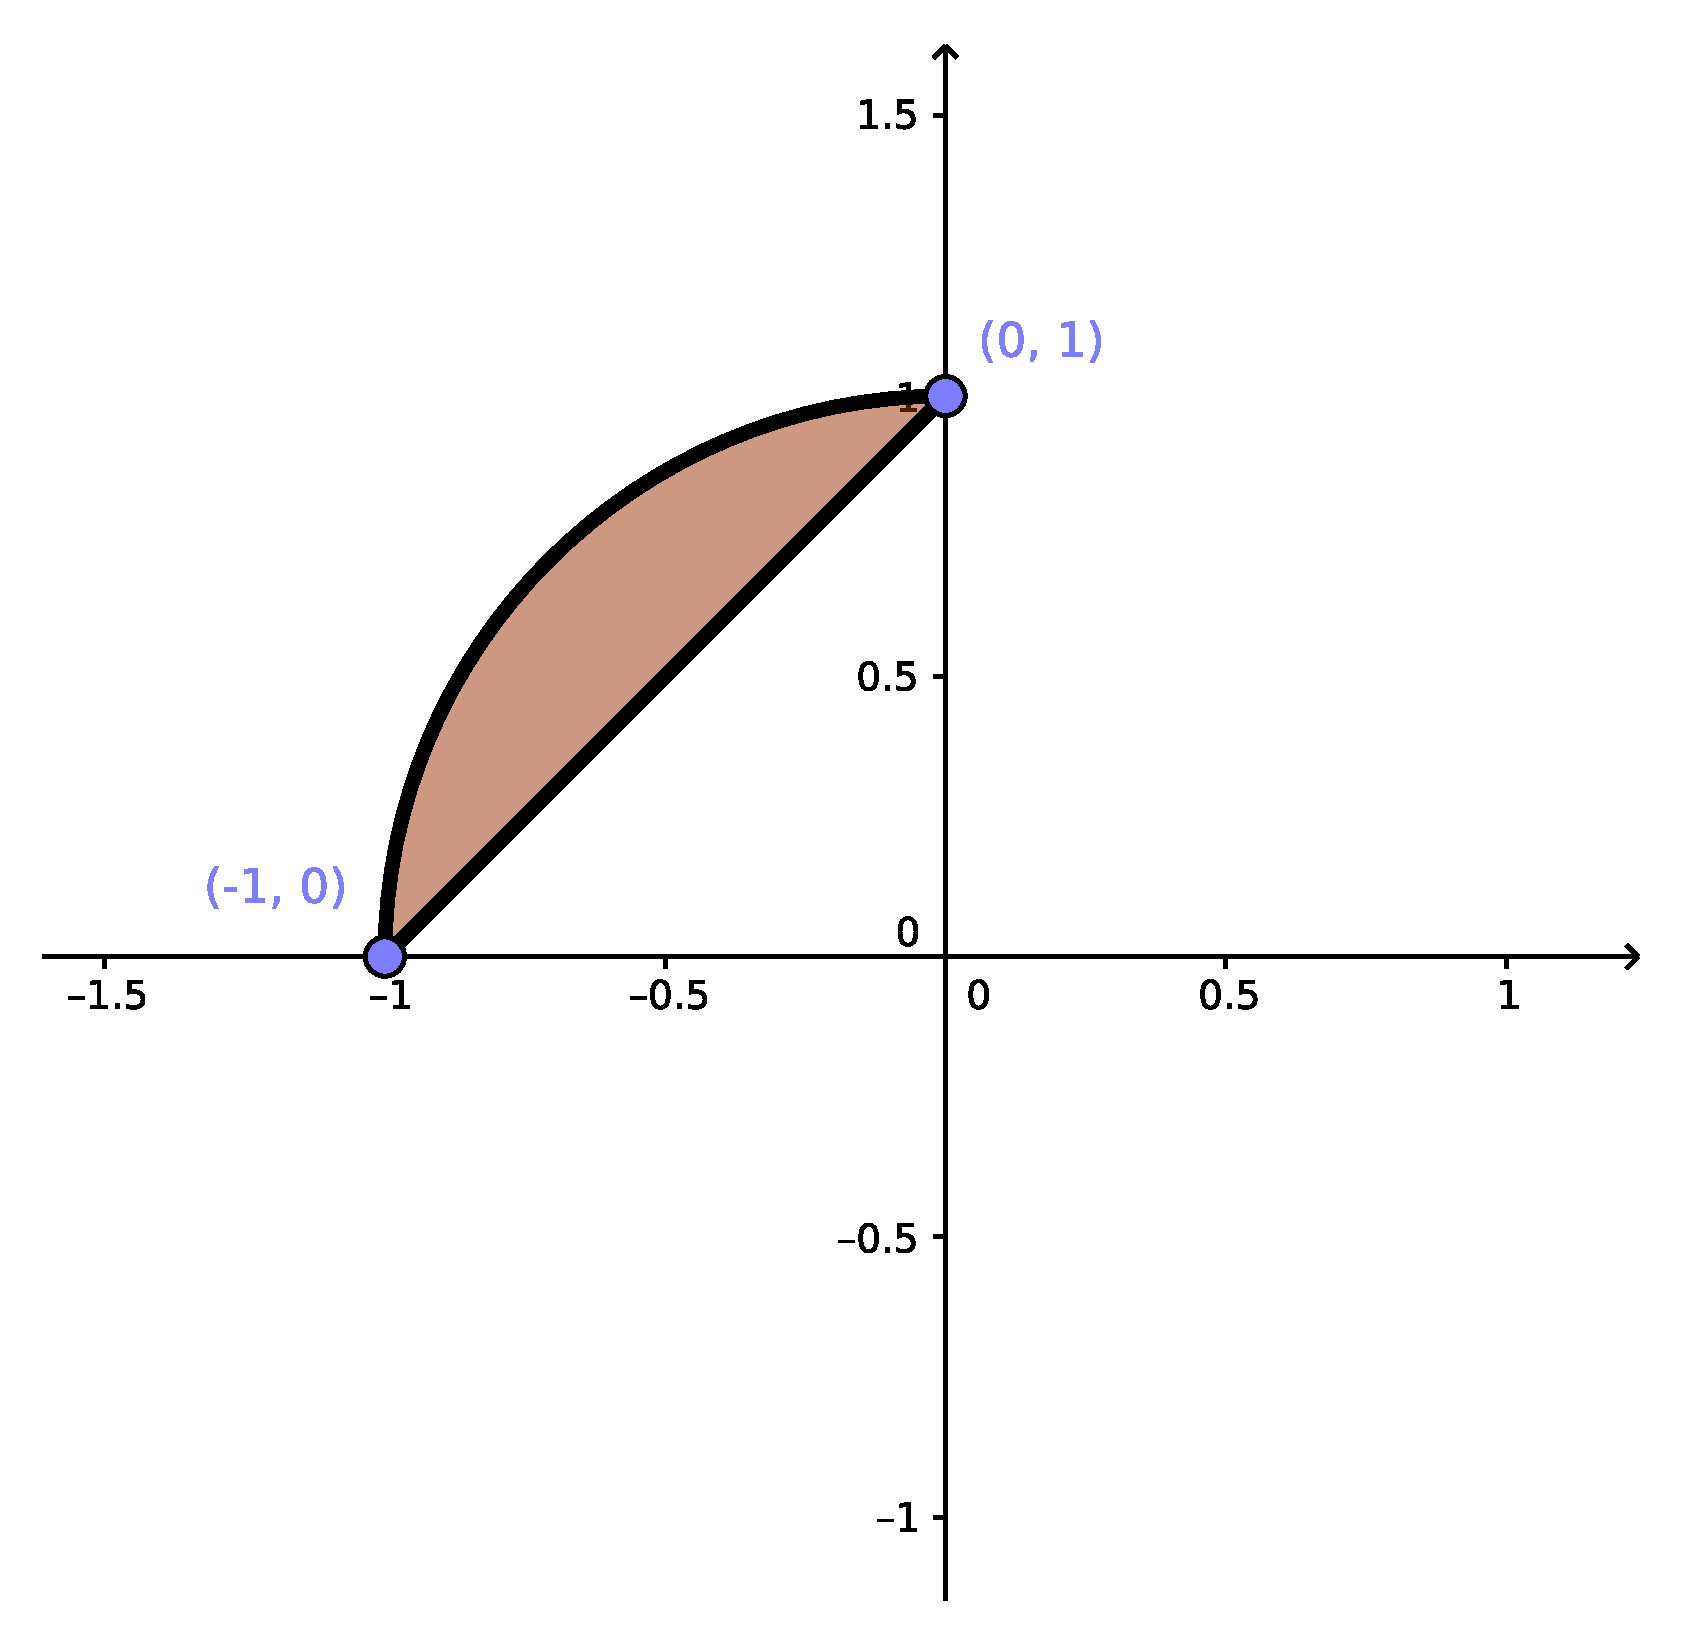
\includegraphics[width=0.45\textwidth]{ex5.pdf}
		\end{figure}
	\vspace{0.5cm}

	\item
		Calcule o trabalho realizado pelo campo vetorial $F(x,y) =
		(4x^3y^2-2xy^3, 2x^4y-3x^2y^2+4y^3)$ ao mover uma part\'{\i}cula ao longo do caminho
		$r(t) = (\cos(t), \sen(t))$, $0\le t \le \pi$.

\end{enumerate}

\begin{flushright}
	\textit{Boa Prova!}
\end{flushright}

\end{document}
